\begin{frame}
  \frametitle{Blockchain}
  \framesubtitle{What is it?}

\begin{columns}
\begin{column}{0.5\textwidth}
  \begin{center}
   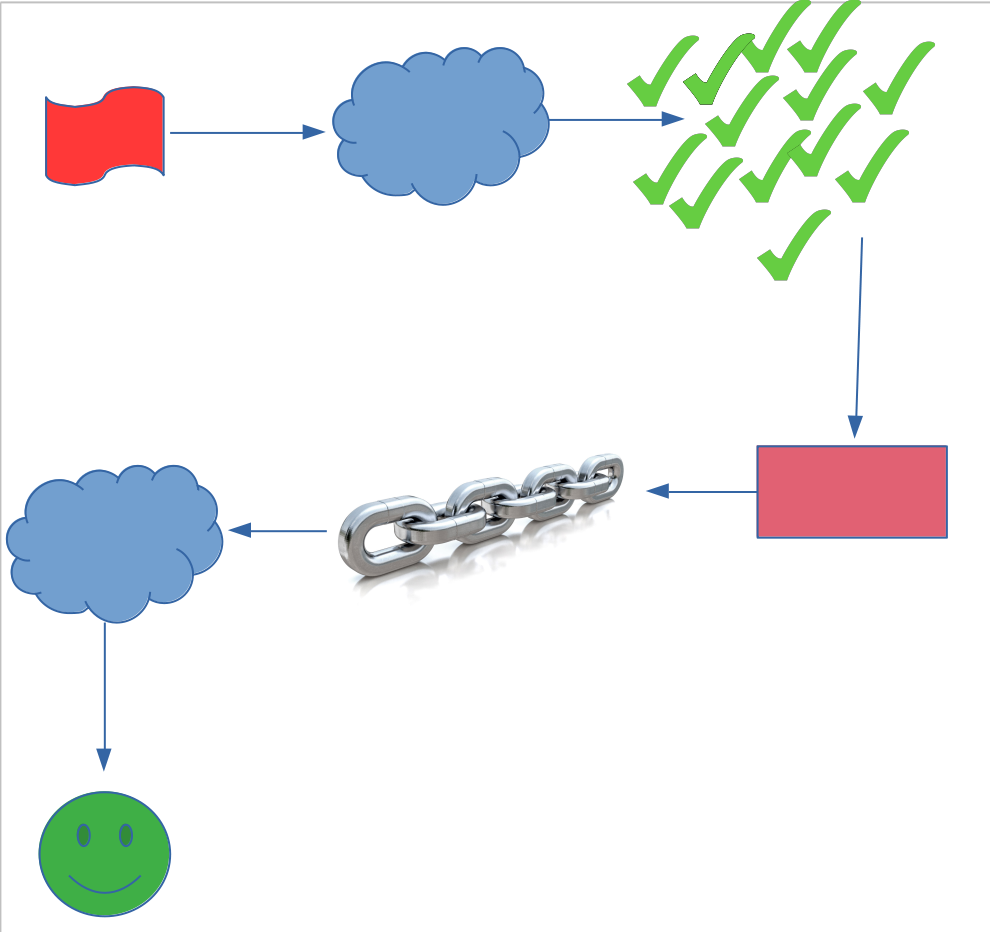
\includegraphics[width=0.9\textwidth]{blockchain}
   \end{center}
\end{column}
\begin{column}{0.5\textwidth}  %%<--- here

          \begin{enumerate}
\scriptsize
            \item A transaction is created
            \item It is sent to a cloud of hundreds, thousands or millions of users
            \item The users all validates the transaction
            \item The validated transaction is encrypted as a block
            \item The block is added to the chain in a way that can not be altered
            \item The block is distributed to the cloud
            \item The transaction is now complete
            \item The system is ready for the next transaction
                 \end{enumerate}
\end{column}
\end{columns}

\end{frame}
